\documentclass [10pt]{article}
\textheight	8.7in
\textwidth	6.5in
\topmargin	    0in
\oddsidemargin  0in
\evensidemargin 0in
\baselineskip 15pt

\usepackage{amssymb,amsmath,amstext}
\usepackage{amsfonts}
\usepackage{mathtools}
\usepackage{tikz}
\usetikzlibrary{automata,arrows,calc,positioning}

\begin{document}
\title{Theory of Computation Assignment no. 6}
\author{Goktug Saatcioglu}
\date{}
\maketitle

\begin{enumerate}
	\item[\textbf{(1)}]$A = \{a^{i}b^{j}\:|\:i\ne j^{2}\}$. Let $x = a^{i^{2}}$ where $i \ge 0$ and $y = a^{j^{2}}$ where $j \ge 0$. If $i \ne j$, we claim that $x$ and $y$ are not equivalent with respect to $A$. Let $z = b^{j}$, then $xz \in A$ but $yz \notin A$. Thus, $x$ and $y$ are not equivalent and $A$ has an infinite number of non-equivalent words with respect to $A$. Therefore, $A$ is not regular. 
	\item[\textbf{(2)}]
	\begin{enumerate}
		\item[a.]Assume that $w \sim_{A} w^{\prime}$ which means $[w]_{A}=[w^{\prime}]_{A}$. Now consider the extension of $\delta$, the $\delta^{*}$ function for $\delta^{*}([\lambda]_{A},wa)$ where $w\in\Sigma^{*}$ and $a\in\Sigma$.
		\begin{align}
			\delta^{*}([\lambda]_{A},wa) &= \delta(\delta^{*}([\lambda]_{A},w),a) && \text{by definition of $\delta^{*}$} \nonumber \\
			&= \delta(\delta^{*}([\lambda]_{A},w^{\prime}),a) && \text{by our assumption that $w \sim_{A} w^{\prime}$} \nonumber \\
			&= \delta^{*}([\lambda]_{A},w^{\prime}a) && \text{by definition of $\delta^{*}$} \nonumber \\
			&\implies [wa]_{A} = [w^{\prime}a]_{A} \implies wa \sim_{A} w^{\prime} \nonumber
		\end{align}
		Thus, we have shown that for any $w\in\Sigma^{*}$, if $w\sim w^{\prime}$ then for every $a\in\Sigma$ it also holds that $wa\sim_{A}w^{\prime}a$. The intuition behind this is if we run a DFA $M$ on words $w$ and $w^{\prime}$ from the initial state independently from each other they will end up in the same state if the words are equivalent with respect to $M$. Since we assume that $w \sim_{A} w^{\prime}$ we know that when $M$ is run on $w$ and $w^{\prime}$ from the initial state independently from each other, they will end up in the same state. Then for all $a\in\Sigma$, if we run $a$ they should again end up in the same state as there is only a single transition to take because M is a DFA. Thus, running $M$ on $wa$ and $w^{\prime}a$ will also end up in the same state if $w\sim_{A}w^{\prime}$.
		\item[b.]We show that $\delta^{*}([\lambda]_{A},w)=[w]_{A}$ for every $w\in\Sigma^{*}$ using induction on the length of $w$, say $n$.\\
		\textbf{Base cases.}\\
		$n=0\implies\left|w\right|=0\implies w=\lambda$.
		\begin{align}
			\delta^{*}([\lambda]_{A},w) &= \delta^{*}([\lambda]_{A},\lambda) && \text{$w=\lambda$} \nonumber \\
			&= q_{0} && \text{by definition of $\delta^{*}$} \nonumber \\
			&= [\lambda]_{A} && \text{since $q_{0}=[\lambda]_{A}$} \nonumber \\
			&= [w]_{A} && \text{since $\lambda=w$} \nonumber
		\end{align}
		$n=1\implies\left|w\right|=1\implies w=a$.
		\begin{align}
			\delta^{*}([\lambda]_{A},w) &= \delta^{*}([\lambda]_{A},a) && \text{$w=a$} \nonumber \\
			&= [\lambda a]_{A} && \text{by definition of $\delta^{*}$} \nonumber \\
			&= [a]_{A} \nonumber \\
			&= [w]_{A} && \text{since $a=w$} \nonumber
		\end{align}
		Since $LHS = RHS$ for both cases, the base cases hold.\\
		\textbf{Inductive step.} For some $n\ge0$, assume that $\delta^{*}([\lambda]_{A},w)=[w]_{A}$ where $\left|w\right|=n$. Now for $k=n$, consider a $w^{\prime}$ such that $\left|w^{\prime}\right|=k+1$ and $w^{\prime}=wa$, where $w\in\Sigma^{*}$ such that $\left|w\right|=k$ and $a\in\Sigma$. Now we evaluate $\delta^{*}([\lambda]_{A},w^{\prime})$.
		\begin{align}
			\delta^{*}([\lambda]_{A},w^{\prime}) &= \delta^{*}([\lambda]_{A},wa) && \text{$w^{\prime}=wa$} \nonumber \\
			&= \delta(\delta^{*}([\lambda]_{A},w),a) && \text{by definition of $\delta^{*}$} \nonumber \\
			&= \delta([w]_{A},a) && \text{by the induction hypothesis} \nonumber \\
			&= [wa]_{A} && \text{by definition of $\delta$} \nonumber \\
			&= [w^{\prime}]_{A} && \text{$wa=w^{\prime}$} \nonumber
		\end{align}
		\textbf{Conclusion.} By the principle of induction, we see that for every $w\in\Sigma^{*}$, $\delta^{*}([\lambda]_{A},w)=[w]_{A}$. $\Box$
	\end{enumerate}
	\item[\textbf{(3)}]
	\begin{enumerate}
		\item[(iii)]The sequence of vertices and associated data configurations the PDA goes through in a recognizing computation on input $abba$ is as follows:
		$$\xrightarrow[]{}p\xrightarrow[\text{Push $\$$}]{\text{$\lambda$}}q\xrightarrow[\text{Push $A$}]{\text{Read $a$}}q\xrightarrow[\text{Pop $A$}]{\text{Read $b$}}q\xrightarrow[\text{Pop $\$$, Push $\$$}]{\text{$\lambda$}}r\xrightarrow[\text{Push $B$}]{\text{Read $b$}}r\xrightarrow[\text{Pop $A$}]{\text{Read $a$}}r\xrightarrow[\text{Pop $\$$}]{\text{$\lambda$}}s.$$
		There are other computation paths that can be followed on this input but they are trivial paths. One such path would be:
		$$\xrightarrow[]{}p\xrightarrow[\text{Push $\$$}]{\text{$\lambda$}}r\xrightarrow[\text{Pop $\$$, Push $\$$}]{\text{$\lambda$}}q\xrightarrow[\text{Push $A$}]{\text{Read $a$}}q\xrightarrow[\text{Pop $A$}]{\text{Read $b$}}q\xrightarrow[\text{Pop $\$$, Push $\$$}]{\text{$\lambda$}}r\xrightarrow[\text{Push $B$}]{\text{Read $b$}}r\xrightarrow[\text{Pop $A$}]{\text{Read $a$}}r\xrightarrow[\text{Pop $\$$}]{\text{$\lambda$}}s.$$
		Many similar such paths can be created by performing trivial operations until getting to $q$ and performing the Read $a$, Push $A$ operation, then performing such trivial operations between $q$ and $r$ before performing the Read $b$, Push $B$ operation and then finally looping back and forth between $q$ and $r$ without reading anything until we choose to get to $s$ using Pop $\$$. Even though these paths are trivial, they are possible and valid.
		\item[(iv)]The language accepted by this PDA is $\{w\in\{ab,ba\}^{*}\}$.
	\end{enumerate}
	\item[\textbf{(4)}]
	\begin{enumerate}
		\item[(i)]Consider the following PDA\\
		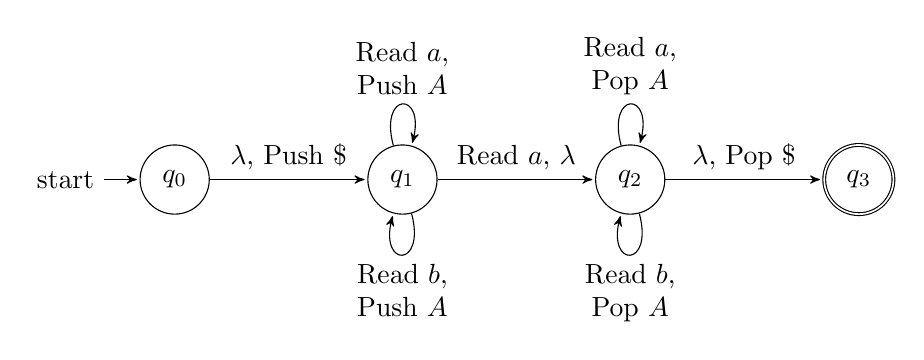
\begin{tikzpicture}[baseline=(q_0.north),>=stealth',shorten >=1pt, auto,node distance=2.0cm,align=center]
			\node[state,initial] (q_0) {$q_{0}$};
			\node[state] [right=of q_0] (q_1) {$q_{1}$};
			\node[state] [right=of q_1] (q_2) {$q_{2}$};
			\node[state,accepting] [right=of q_2] (q_3) {$q_{3}$};
			\path[->]
				(q_0) edge node {$\lambda$, Push $\$$} (q_1)
				(q_1) edge [loop above] node {Read $a$,\\Push $A$} ()
				(q_1) edge [loop below] node {Read $b$,\\Push $A$} ()
				(q_1) edge node {Read $a$, $\lambda$} (q_2)
				(q_2) edge [loop above] node {Read $a$,\\Pop $A$} ()
				(q_2) edge [loop below] node {Read $b$,\\Pop $A$} ()
				(q_2) edge node {$\lambda$, Pop $\$$} (q_3);
		\end{tikzpicture}\\
		where $q_{0}$ is the empty string $\lambda$ and empty stack, $q_{1}$ reads some $\{a,b\}^{*}$ and the stack contains $\left|q_{1}\right|$ number of $A$'s, $q_{2}$ has read a single $a$ and then reads some $\{a,b\}^{*}$ as the stack empties out $\left|q_{1}\right|$ number of $A$'s, and $q_{3}$ is the empty string $\lambda$ and empty stack with the number of $A$'s pushed in $q_{1}$ equaling the number of $B$'s popped in $q_{2}$. This works since we want an equal number of letters on the right and left of the middle $a$. We use the fact that if the number of letters right and left of $a$ is odd then $w$ is odd and, similarly, if the number of letters right and left of $a$ is even then $w$ is odd. Furthermore, in both cases $a$ will end up in the middle. Thus, this PDA will start pushing a $\$$ (shielding) sign onto the stack and then $A$'s onto the stack for some $n$ number of letters it sees which means the stack will contain $n$ number of $A$'s. When a middle $a$ is seen nothing is pushed or popped from the stack and every letter seen after the middle $a$ will mean we pop an $A$ from the stack. If we can pop $n$ number of letters we will only end up with the $\$$ (shielding) sign on the stack and we can pop this to end up at the accepting state.
		\item[(vi)]Consider the following PDA\\
		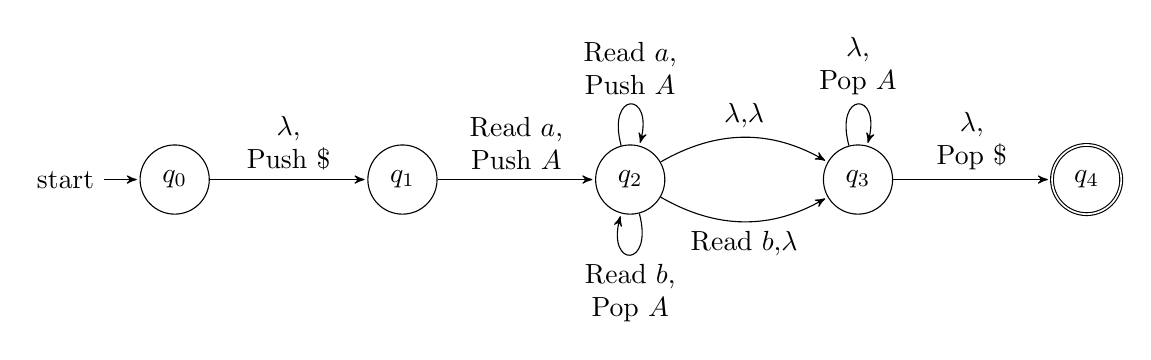
\begin{tikzpicture}[baseline=(q_0.north),>=stealth',shorten >=1pt, auto,node distance=2.0cm,align=center]
			\node[state,initial] (q_0) {$q_{0}$};
			\node[state] [right=of q_0] (q_1) {$q_{1}$};
			\node[state] [right=of q_1] (q_2) {$q_{2}$};
			\node[state] [right=of q_2] (q_3) {$q_{3}$};
			\node[state,accepting] [right=of q_3] (q_4) {$q_{4}$};
			\path[->]
				(q_0) edge node {$\lambda$,\\Push $\$$} (q_1)
				(q_1) edge node {Read $a$,\\Push $A$} (q_2)
				(q_2) edge [loop above] node {Read $a$,\\Push $A$} ()
				(q_2) edge [loop below] node {Read $b$,\\Pop $A$} ()
				(q_2) edge [bend left] node {$\lambda$,$\lambda$} (q_3)
				(q_2) edge [bend right] node [below] {Read $b$,$\lambda$} (q_3)
				(q_3) edge [loop above] node {$\lambda$,\\Pop $A$} ()
				(q_3) edge node {$\lambda$,\\Pop $\$$} (q_4);
		\end{tikzpicture}\\
		where $q_{0}$ is the empty string $\lambda$ and empty stack, $q_{1}$ is the state where the shielding symbol $\$$ is pushed onto the stack and a first $a$ is read such that $A$ is pushed onto the stack (the necessity of this is explained below), $q_{2}$ reads some amount of $a$'s and $b$'s and pushs $A$ onto the stack for every $a$ and pops $A$ from the stack for every $b$ such that for every initial string $\#a(w) \ge \#b(w)$, $q_{3}$ is the state where a final letter is read and now we can keep popping $A$'s until we get to the shielding symbol, and $q_{4}$ is the empty string and empty stack where we have recognized the language specified by the question.
		The way I interpreted this question is that for every $1 \le k < \left|w\right|$ length "initial string" of $w$, (i.e. $abab$ has initial strings $a$, $ab$, and $aba$) $\#a(w) \ge \#b(w)$. For us to recognize this language we need to ensure that every inputs starts with an $a$ and we count the occurrence of this $a$ by pushing an $A$ onto the stack. In this case we don't need to use shielding and the reason for this will be explained below. Then for every next $a$ we see we push an $a$ and for every next $b$ we see we pop a $B$. This gaurantees that as we read letters $\#a(w) \ge \#b(w)$ and something like $abb$ will not be recognized by the PDA. However, we know that $aabbb$ should be recognized as the whole word $w$ is not an initial string and thus, we add a $\lambda$ transition for reading a $b$ that takes us to the state where we can continually pop $A$'s until we get to the shielding symbol. In this state, if we can't pop $A$'s until we get to $\$$, then we know that the word is not in the language and otherwise we pop $\$$ and get to the accepting state.
	\end{enumerate}
	\item[\textbf{(5)}]
		\begin{enumerate}
			\item[(v)]The set of strings generated by this grammar involve the concatenation of two different set of strings. The first set is the set of strings such that there are some $j$ amount of words in the form $c^{j}d^{j}$ where $j$ can be $0$ which is preceeded by $m$ amount of $a$'s and suceeded by $i$ amount of $b$'s where $i$ can be $0$. The second set is an $o$ amount of word in the form $c^{k}d^{k}$ where $k$ can be $0$. In terms of set notation, $S$ can be described as$$\{(a^{i}(c^{j}d^{j})b^{i})(c^{k}d^{k})\:|\:i,j,k\ge0\}.$$
		\end{enumerate}
	\item[\textbf{(6)}]
		\begin{enumerate}
			\item[(i)]The context free grammar is as follows:
			\begin{align}
				S &\rightarrow TST\:|\:a \nonumber \\
				T &\rightarrow a\:|\:b \nonumber
			\end{align}
		\end{enumerate}
\end{enumerate}

\end{document}